\documentclass{article}
\usepackage[utf8]{inputenc}
\usepackage{amsmath}
\usepackage{amsfonts}
\usepackage[margin=0.7in]{geometry}
\usepackage{graphicx}
\usepackage{amssymb}
\usepackage{gensymb}
\usepackage{booktabs}
\usepackage{wrapfig}
\usepackage{caption}
\usepackage[export]{adjustbox}
\usepackage[pdfborder={0 0 0}]{hyperref}
\usepackage{pdfpages}
\usepackage{fancyhdr}
\usepackage{parskip}
\usepackage{lastpage}
\usepackage{listings}
\usepackage{multirow}
\usepackage{xifthen}
\usepackage{xcolor}
\graphicspath{{Images/}} 
\pagestyle{fancy}
\title{Aflevering 5i}
\usepackage{natbib}

\begin{document}
\author{Carl-Emil Rohde }
\maketitle

\section*{Problemformulering}
I denne opgave skal der i et dotnet projekt implementeres moduler, der indeholder funktioner, som udførerer en række forskellige handlinger på den abstrakte datatype "queues". Der implementeres løsninger der fortæller hvad en funktion skal gøre, hvis den bliver kaldt med en tom liste. I første del af opgaven, arbejdes der med queues' af heltal, hvorefter der senere i opgaven implementeres moduler, der kan arbejde med queues af alle datatyper.  


\section*{Løsningsovervejelser}
\subsection*{5i0}
I denne opgave har jeg oprettet den overordnet filstruktur i dotnet, hvor projektfilen, implementerings- og programfilenerne skal ligge. Jeg har givet mappen navnet 5i.  

\subsection*{5i1}
I denne opgave har jeg oprettet et modul kaldet "IntQueue". Jeg har oprettet en implementerings og signaturfil med samme navn, som indeholder fire forskellige funktioner, der hver især foretager forskellige operationer på queue elementerne. 

Herunder følger en kort beskrivelse af hver funktion:

"emptyQueue" tager ingen parametre, og laver blot en ny tom queue. 

"enqueue" tager to parametre, hhv en queue og et heltal, sætter de to ting sammen, og returnerer en ny queue. 

"isEmpty" tager en queue som parametre, tjekker om den er tom, og returnerer så et true/false-statement afhængig af udfaldet. 

"dequeue" tager også en queue som parametre, returnerer det øverste element i den queue, samt den resulterende queue.  

Jeg har kørt funktionerne igennem testprogrammet fra opgavebeskrivelsen, som jeg har kopieret ind i en fil kaldet "testQueues.fs". Herunder ses resultatet: 

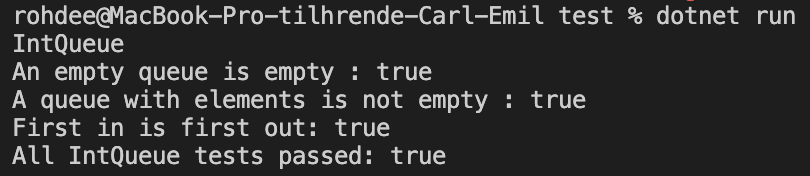
\includegraphics[scale=0.85]{5i1test.png}


\subsection*{5i2}
I denne opgave, skal jeg udvide dequeue funktionen fra forrige opgave, så man ikke ved en fejl kan komme til at kalde funktionen med en tom queue, da dequeue kun fungererer korrekt på en queue med ét eller flere elementer. Denne implementering har jeg lavet, ved at bruge else/if statements og lavet et kald på funktionen "isEmpty" fra forrige opgave, der her fungerer som hjælpe funktion til at tjekke om den kaldte queue er tom eller ej. Hvis isEmpty returnerer true, det vil sige at vores queue er tom, så returnerer funktionen: (None,[]). Hvis udfaldet derimod er false, altså at queue ikke er tom, så fortæstter dequeue funktionen på samme måde som i 5i1. Alle andre funktioner har jeg ikke ændret ved. Jeg har kørt en lignende test på funktionerne i SafeIntQueue modulet, og får følgende: 

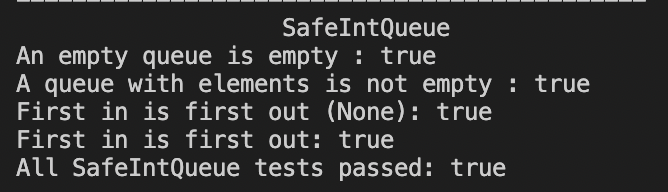
\includegraphics[scale=0.85]{5i22.png}

\subsection*{5i3}
I denne opgave skal jeg udvide funktionerne fra IntQueue modulet, så funktionerne kan foretage operationer på queue's, som ikke blot indholder heltal, men også alle mulige andre typer, som for eksempel; floats, heltal og strings...
Dette har jeg gjort ved at ændre alle typerne til alpha a, altså "'a", samt tilføjet $< 'a >$, til alle queue elementer. Dette gør funktionerne i stand til at behandle forskellige typer af queues. jeg har testet om denne implementering virker, ved i test filen at lave et lille program, der kalder testkoden fra opgavebeskrivelsen med tre forskellige typer, nemlig floats, int's og strings. resultatet giver mig følgende: 

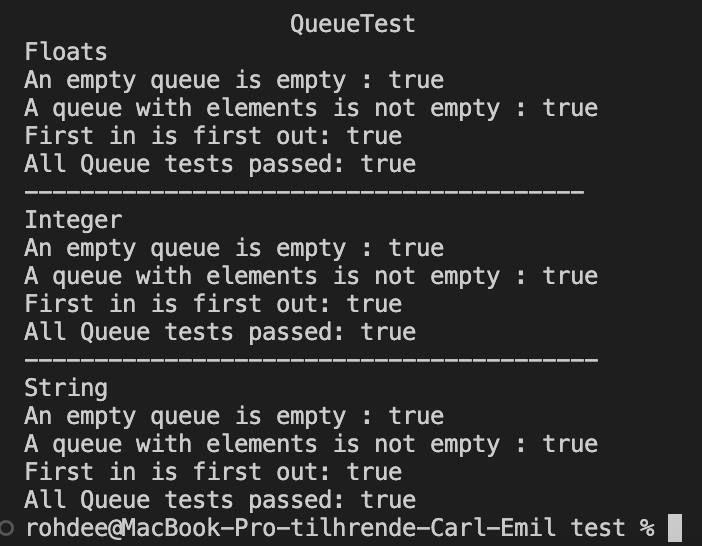
\includegraphics[scale=0.85]{5i3.png}


\end{document}
